\documentclass[11pt]{amsart}          
\usepackage[a4paper,verbose]{geometry}
\geometry{top=3cm,bottom=3cm,left=3cm,right=3cm,textheight=595pt}
\setlength{\parskip}{0.3em}
% ==============================
% PACKAGES
% ==============================

\usepackage{amsfonts}
\usepackage{amssymb}  
\usepackage{amsthm} 
\usepackage{amsmath} 
\usepackage{caption}
\usepackage[inline]{enumitem}
\setlist{itemsep=0em, topsep=0em, parsep=0em}
\setlist[enumerate]{label=(\alph*)}
\usepackage{etoolbox}
\usepackage{stmaryrd} 
\usepackage[dvipsnames]{xcolor}
\usepackage[]{hyperref}
\hypersetup{
  colorlinks,
  linkcolor=blue,
  citecolor=blue,
  urlcolor=blue}
\usepackage{graphicx}
\graphicspath{{assets/}}
\usepackage{mathtools}

\usepackage{tikz-cd}
\usepackage{minted}
\usepackage{float}
\usetikzlibrary{
  matrix,
  arrows,
  shapes
}

\setcounter{tocdepth}{1} % Sets depth for table of contents. 

\newcommand{\rr}{{\mathbb{R}}}
\newcommand{\nn}{{\mathbb{N}}}
\newcommand{\iso}{\cong}
\newcommand{\too}{\longrightarrow}
\newcommand{\tto}{\rightrightarrows}
\newcommand{\To}[1]{\xrightarrow{#1}}
\newcommand{\Too}[1]{\To{\;\;#1\;\;}}
\newcommand{\from}{\leftarrow}
\newcommand{\From}[1]{\xleftarrow{#1}}
\newcommand{\Cat}[1]{\mathbf{#1}}
\newcommand{\cat}[1]{\mathcal{#1}}
\newtheorem*{remark}{Remark}
\renewcommand{\ss}{\subseteq}
\newcommand{\hask}[1]{\mintinline{Haskell}{#1}}
\newenvironment{haskell}
  {\VerbatimEnvironment
  	\begin{minted}[escapeinside=??, mathescape=true,frame=single, framesep=5pt, tabsize=1]{Haskell}}
  {\end{minted}}

\author{Bartosz Milewski}
\title{Adjoint Functor Theorem}

\begin{document}
\maketitle{}

\begin{figure}[H]
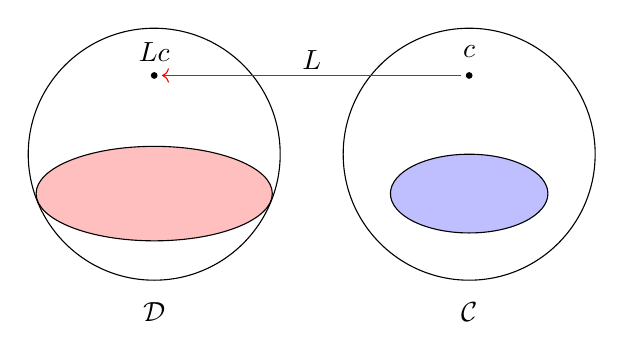
\begin{tikzpicture}
  \def\Xa{-2.0};
  \def\Xb{2.0};
  \def\Yb{-2.0};
  \def\Yp{1.0};
  \def\Yo{-0.5};
         \draw (\Xa, 0) ellipse (1.6 and 1.6);
         \draw (\Xa , \Yo)[fill=red!25!white] ellipse (1.5 and 0.6);
         \draw (\Xb , 0) ellipse (1.6 and 1.6);
         \draw (\Xb , \Yo)[fill=blue!25!white] ellipse (1 and 0.5);
        \node at (\Xa, \Yp + 0.3) { $L c$ };
        \node at ( \Xb, \Yp + 0.3) { $c$ };
        \filldraw (\Xa, \Yp) circle (1pt);
        \filldraw (\Xb, \Yp) circle (1pt);
	\draw[<-, red] (\Xa + 0.1, \Yp) -- (\Xb - 0.1, \Yp);
        \node at (0, \Yp + 0.2) { $L$ };
        \node at (\Xa, \Yb) { $\cat D$ };
        \node at (\Xb, \Yb) { $\cat C$ };
\end{tikzpicture}
\end{figure}

\end{document}


